\chapter{Exemplos de Marcação na Faixa A}
\label{apendice:exemplos}

% Figuras geradas por AI/SAM/figuras_regra_autor.py e copiadas por AI/SAM/figuras_tcc.py.
% Todas as chapas são das vagas de calibração (partição de treinamento): nenhuma vem
% do test/, de onde sai a auditoria (docs/decisoes.md, D7).

As figuras deste apêndice mostram, para cada litotipo da faixa A, as imagens de calibração típica e forte com três painéis lado a lado: a chapa, as marcações no limiar produzido pela regra (Seção \ref{sec:regra}) e as marcações no limiar adotado pelo autor. Os dois painéis de marcação usam as mesmas sondas, as admitidas na descoberta, de modo que a única diferença entre eles é o limiar; em termos do experimento, são os braços de regra com as sondas do autor e calibrado pelo autor (Quadro \ref{quad:bracos_exp1}). O número no topo de cada painel é o de detecções, e a cor indica a sonda que respondeu. As imagens são todas da partição de treinamento; as chapas da auditoria não aparecem aqui. Os litotipos identificados como movimentados (Seção \ref{sec:movimentadas}) estão marcados com $^{\dagger}$.

\begin{figure}[htbp]
  \caption{Regra e autor na \textit{golden\_storm}$^{\dagger}$: imagem típica (acima) e forte (abaixo).}
  \label{fig:ex_ap_golden_storm}
  \centering
  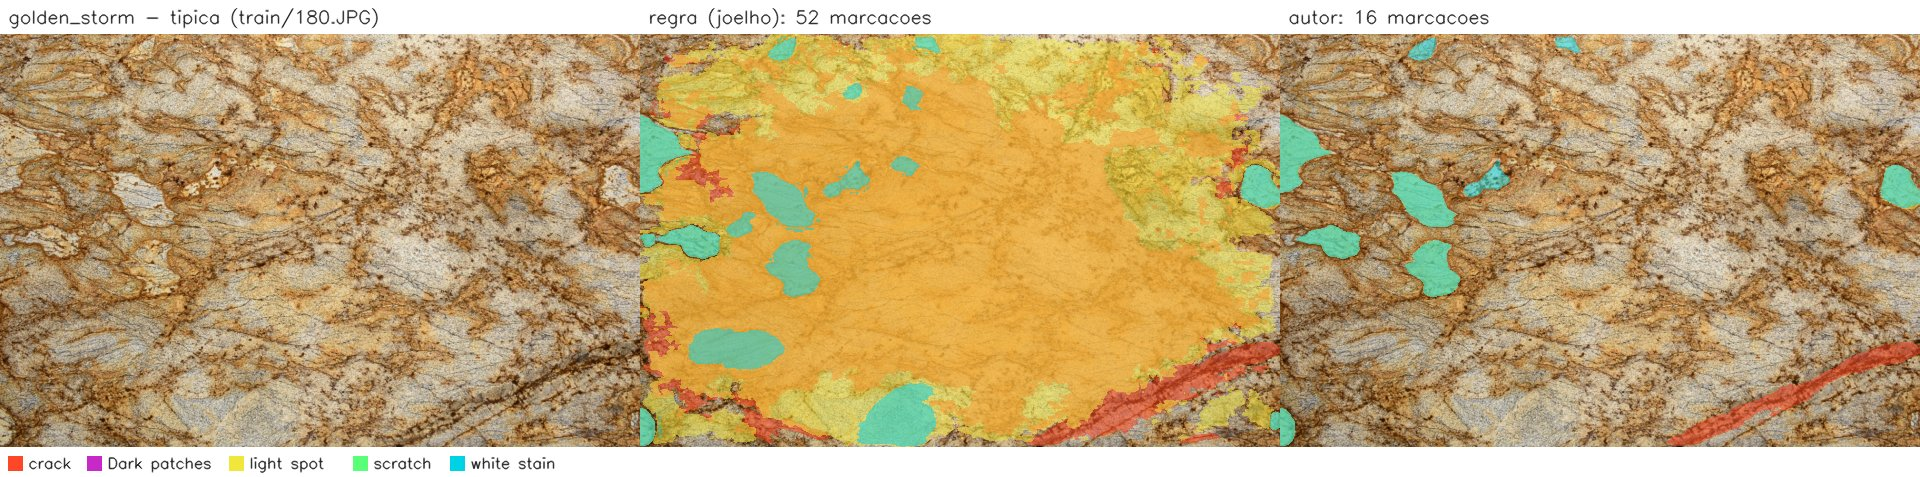
\includegraphics[width=\textwidth]{exemplo_golden_storm_tipica.jpg}

  \vspace{0.4cm}
  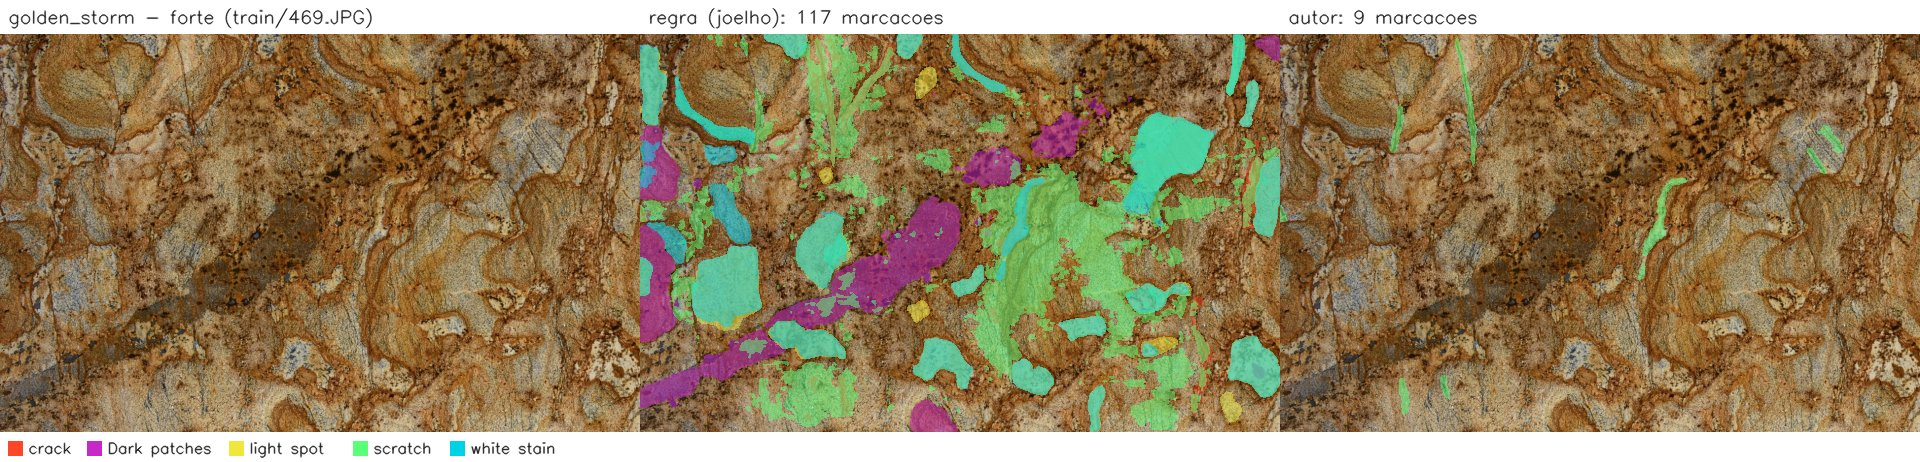
\includegraphics[width=\textwidth]{exemplo_golden_storm_forte.jpg}
  \legend{elaborado pelo autor, sobre imagens de \citeonline{dataset_araujo2023}}
\end{figure}

\begin{figure}[htbp]
  \caption{Regra e autor na \textit{ipanema\_beige}: imagem típica (acima) e forte (abaixo).}
  \label{fig:ex_ap_ipanema_beige}
  \centering
  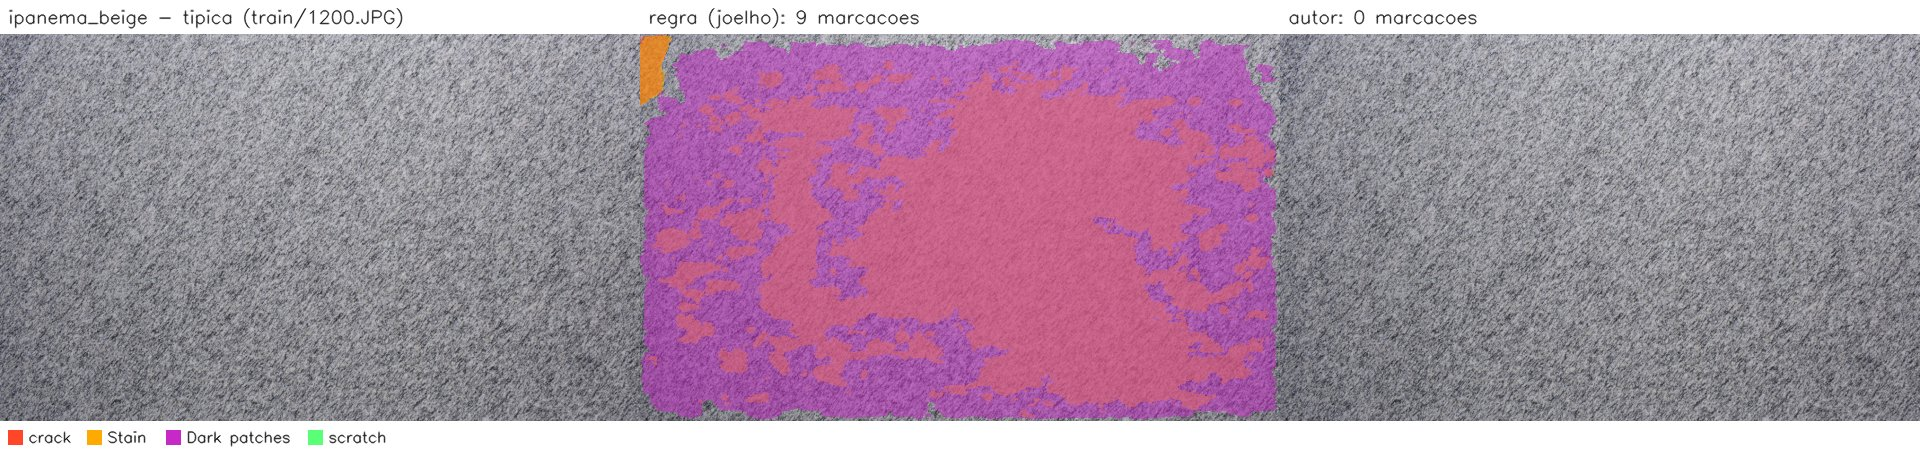
\includegraphics[width=\textwidth]{exemplo_ipanema_beige_tipica.jpg}

  \vspace{0.4cm}
  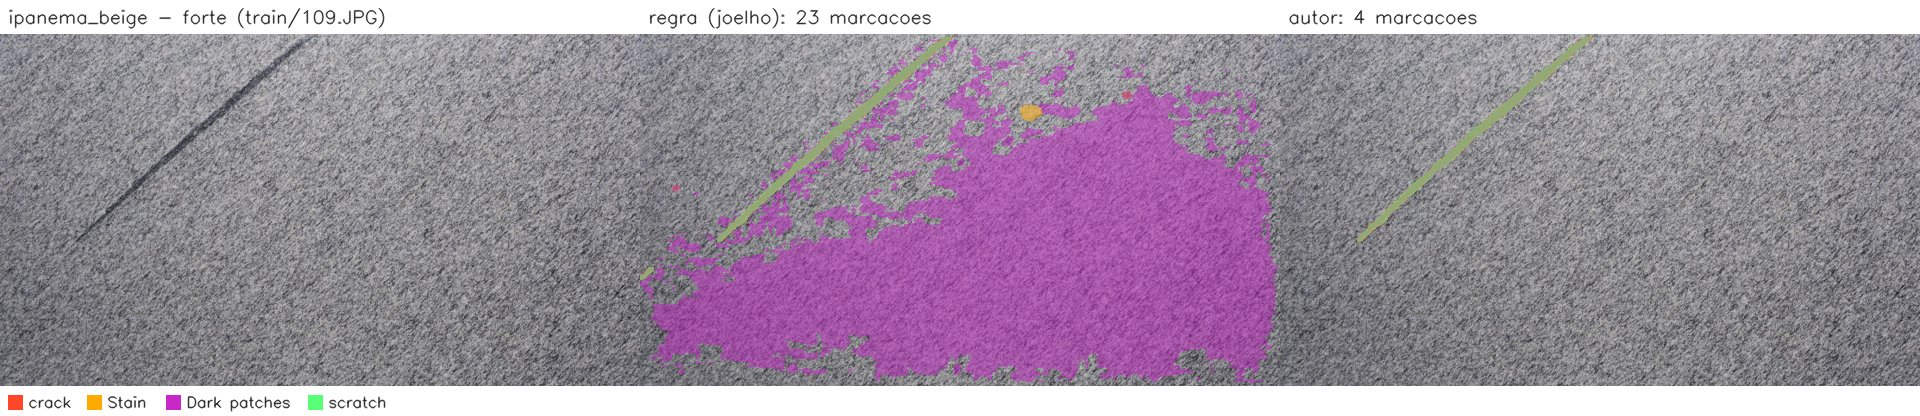
\includegraphics[width=\textwidth]{exemplo_ipanema_beige_forte.jpg}
  \legend{elaborado pelo autor, sobre imagens de \citeonline{dataset_araujo2023}}
\end{figure}

\begin{figure}[htbp]
  \caption{Regra e autor na \textit{itaunas\_white}: imagem típica (acima) e forte (abaixo).}
  \label{fig:ex_ap_itaunas_white}
  \centering
  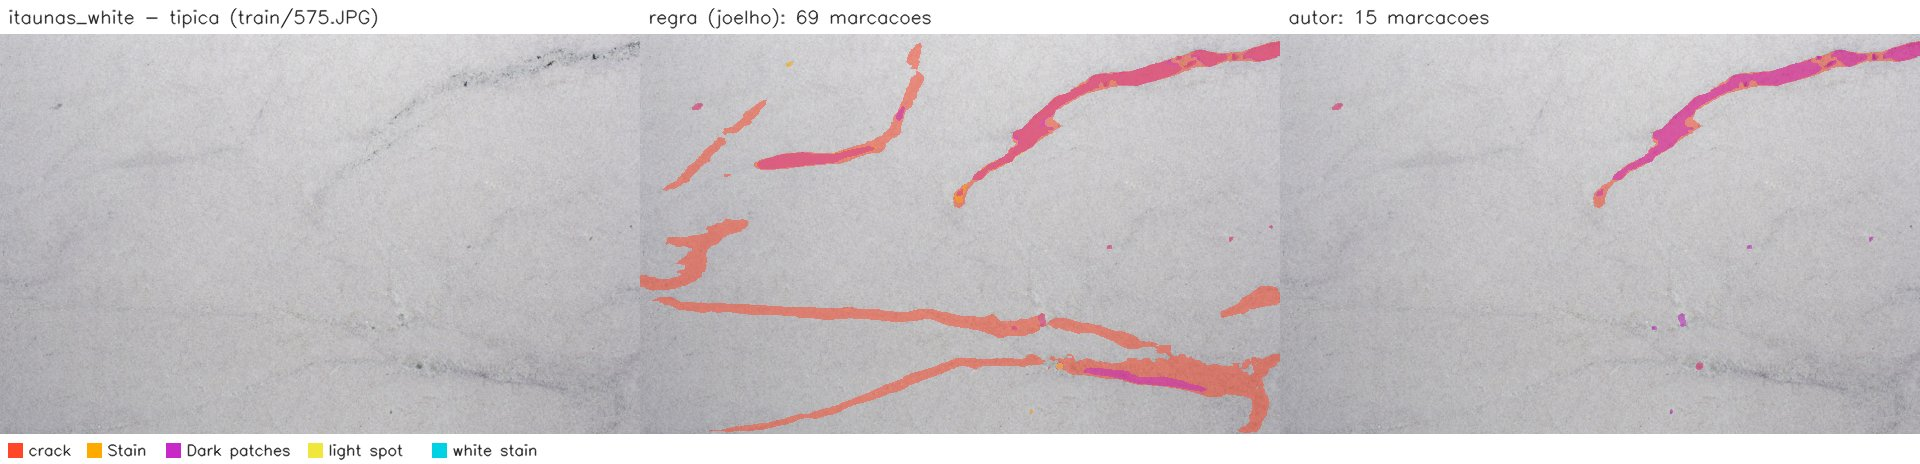
\includegraphics[width=\textwidth]{exemplo_itaunas_white_tipica.jpg}

  \vspace{0.4cm}
  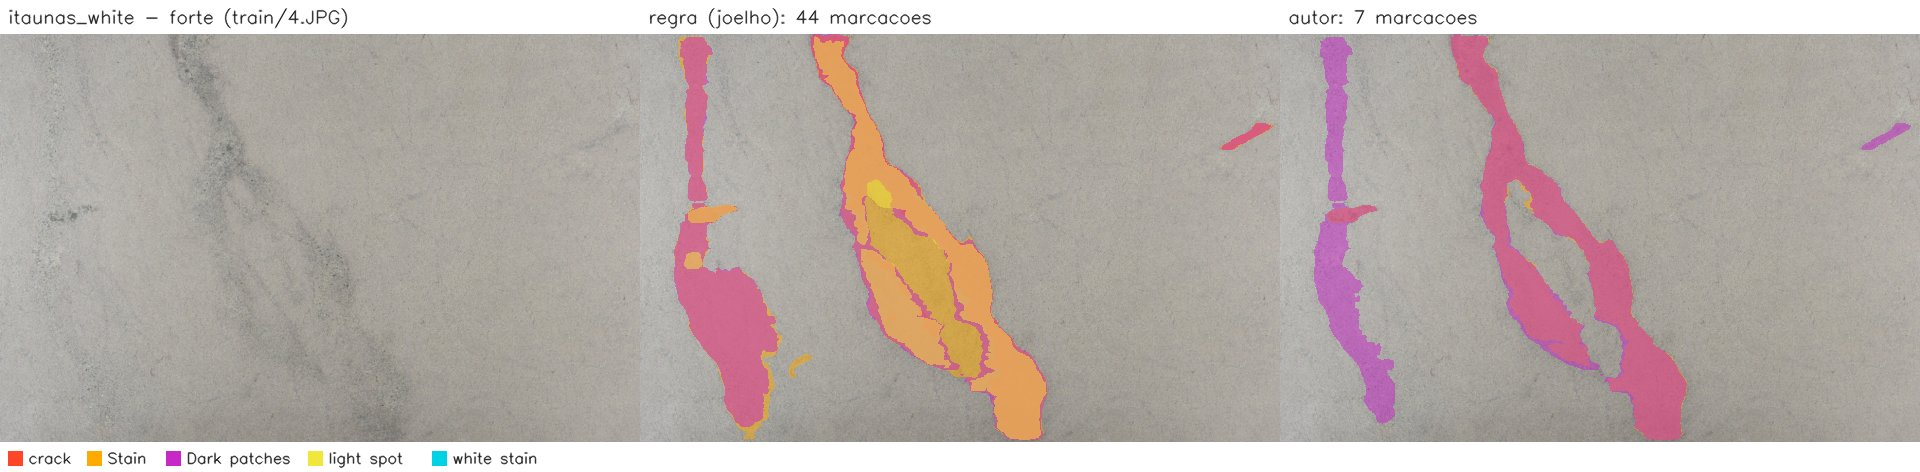
\includegraphics[width=\textwidth]{exemplo_itaunas_white_forte.jpg}
  \legend{elaborado pelo autor, sobre imagens de \citeonline{dataset_araujo2023}}
\end{figure}

\begin{figure}[htbp]
  \caption{Regra e autor na \textit{nevada\_black}: imagem típica (acima) e forte (abaixo).}
  \label{fig:ex_ap_nevada_black}
  \centering
  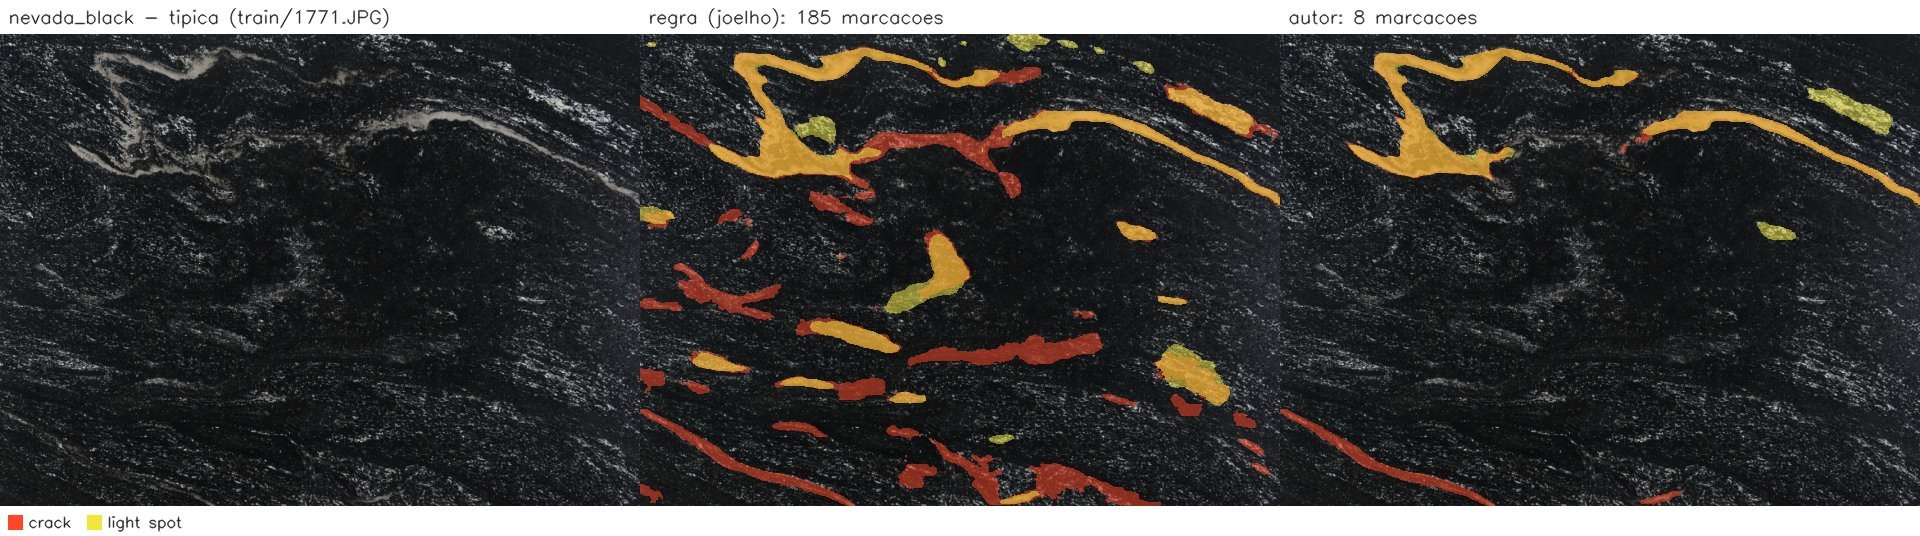
\includegraphics[width=\textwidth]{exemplo_nevada_black_tipica.jpg}

  \vspace{0.4cm}
  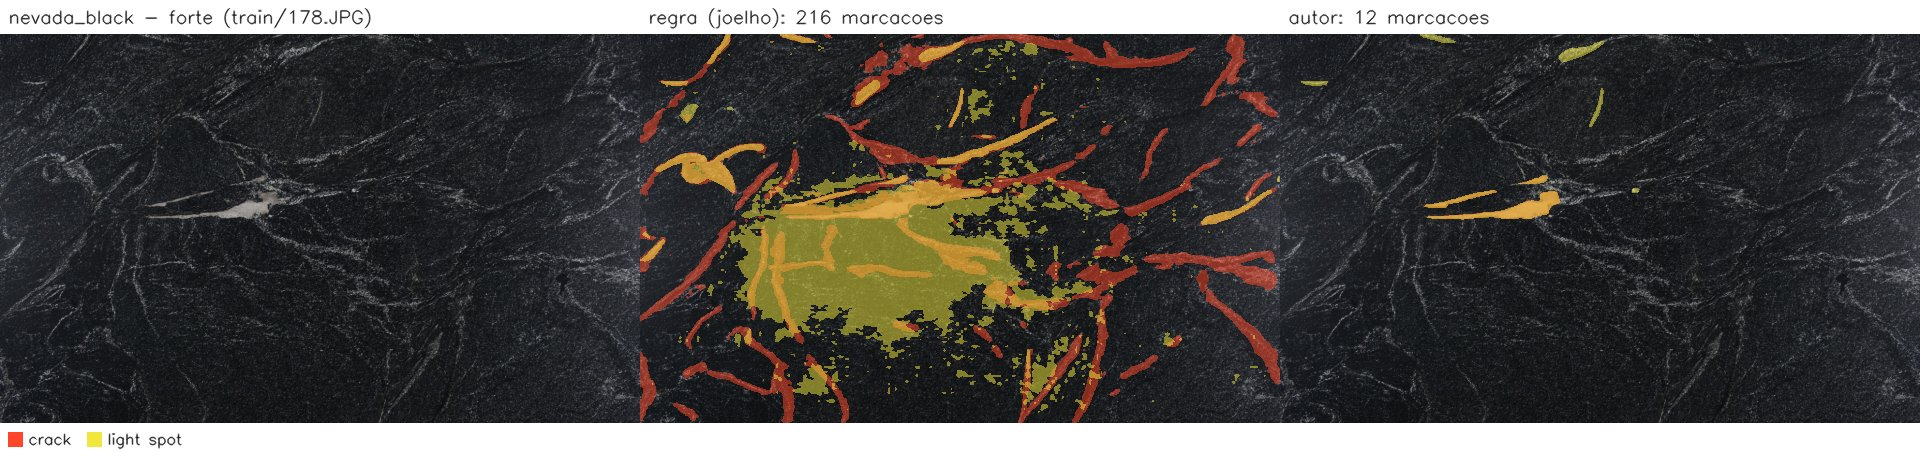
\includegraphics[width=\textwidth]{exemplo_nevada_black_forte.jpg}
  \legend{elaborado pelo autor, sobre imagens de \citeonline{dataset_araujo2023}}
\end{figure}

\begin{figure}[htbp]
  \caption{Regra e autor na \textit{san\_francisco\_green}$^{\dagger}$: imagem típica (acima) e forte (abaixo).}
  \label{fig:ex_ap_san_francisco_green}
  \centering
  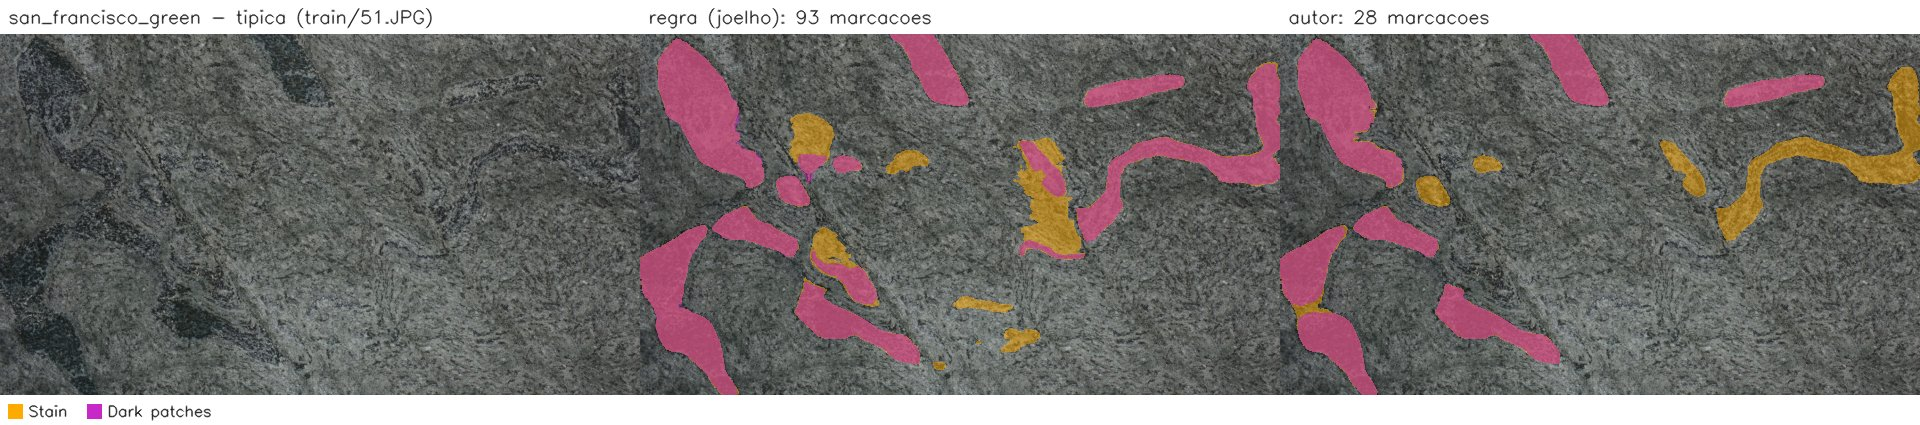
\includegraphics[width=\textwidth]{exemplo_san_francisco_green_tipica.jpg}

  \vspace{0.4cm}
  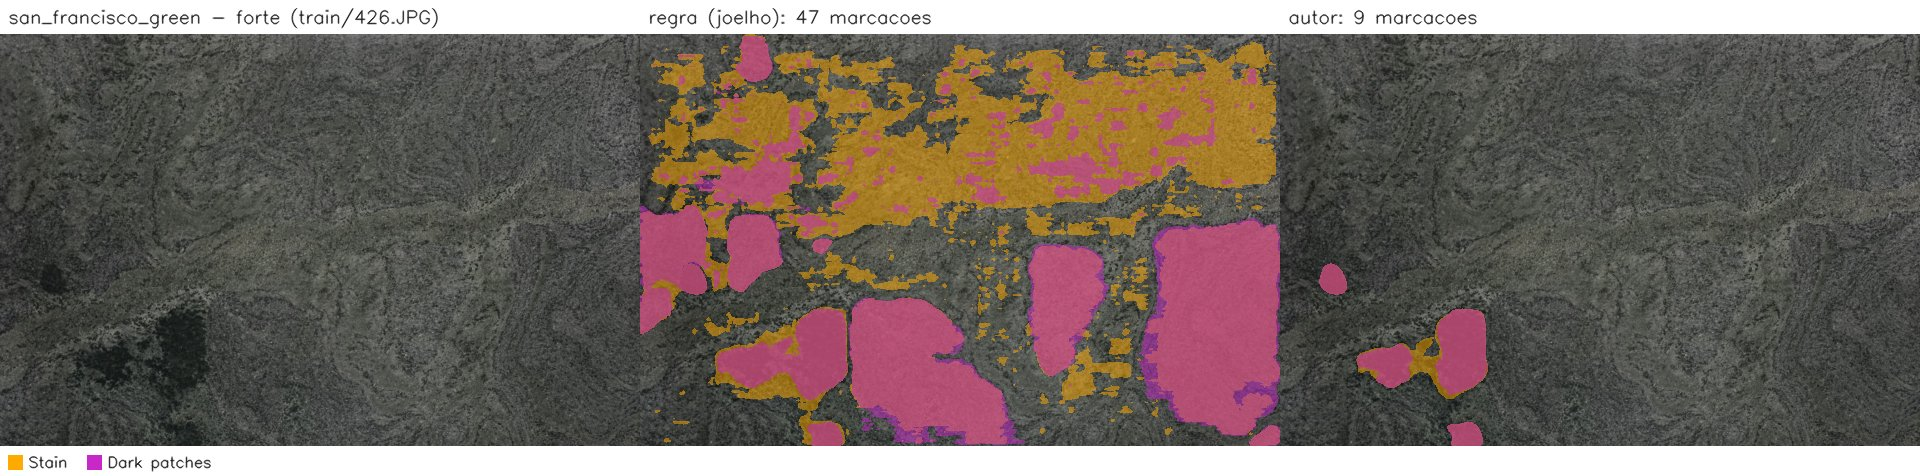
\includegraphics[width=\textwidth]{exemplo_san_francisco_green_forte.jpg}
  \legend{elaborado pelo autor, sobre imagens de \citeonline{dataset_araujo2023}}
\end{figure}

\begin{figure}[htbp]
  \caption{Regra e autor na \textit{santa\_cecilia}: imagem típica (acima) e forte (abaixo).}
  \label{fig:ex_ap_santa_cecilia}
  \centering
  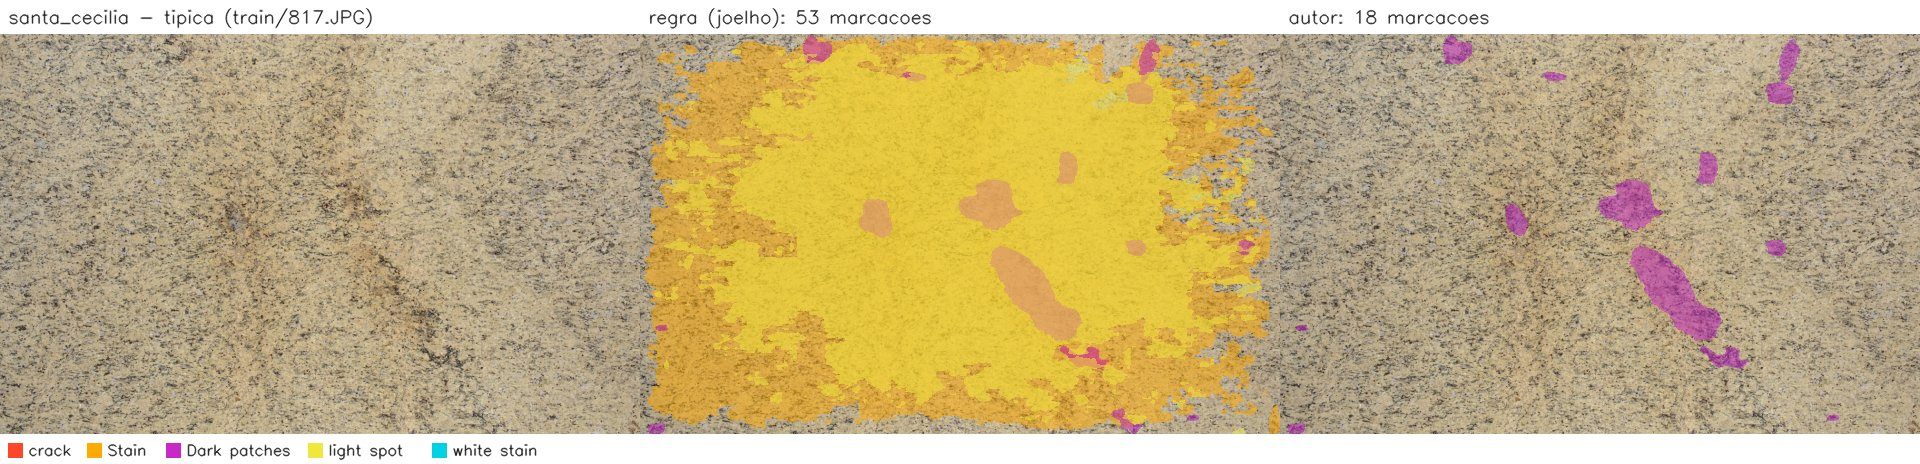
\includegraphics[width=\textwidth]{exemplo_santa_cecilia_tipica.jpg}

  \vspace{0.4cm}
  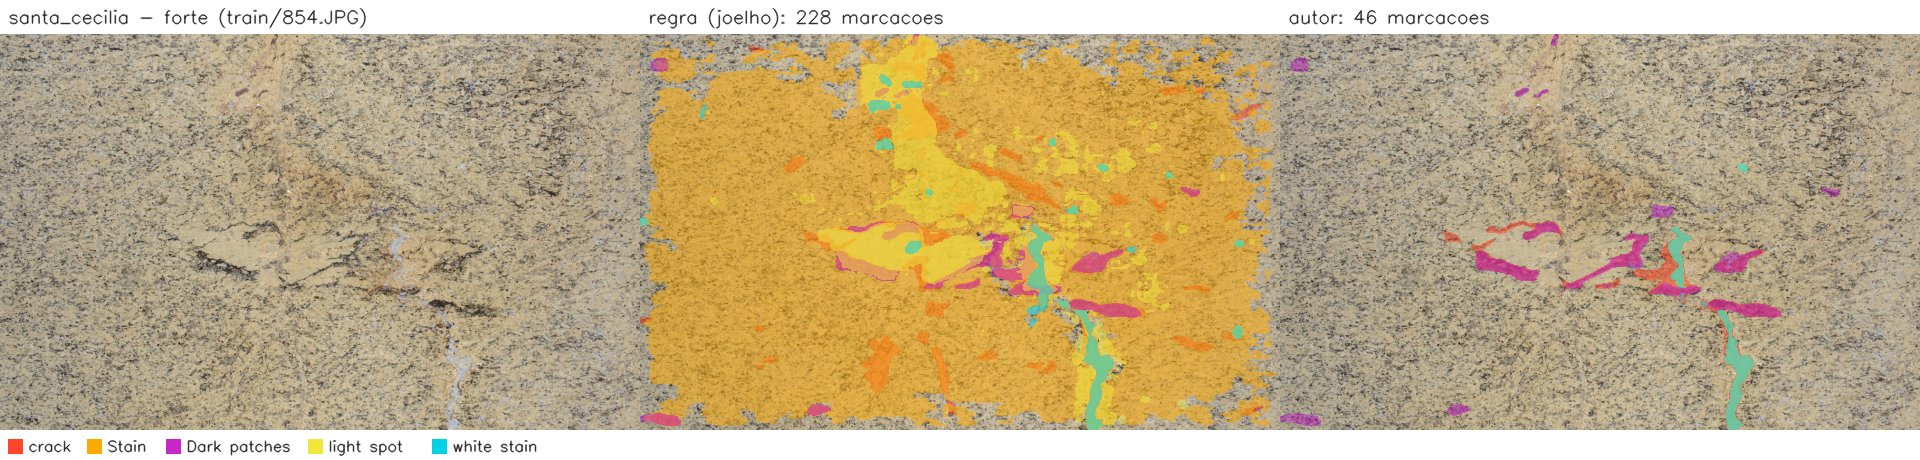
\includegraphics[width=\textwidth]{exemplo_santa_cecilia_forte.jpg}
  \legend{elaborado pelo autor, sobre imagens de \citeonline{dataset_araujo2023}}
\end{figure}

\begin{figure}[htbp]
  \caption{Regra e autor na \textit{shadow\_white}$^{\dagger}$: imagem típica (acima) e forte (abaixo).}
  \label{fig:ex_ap_shadow_white}
  \centering
  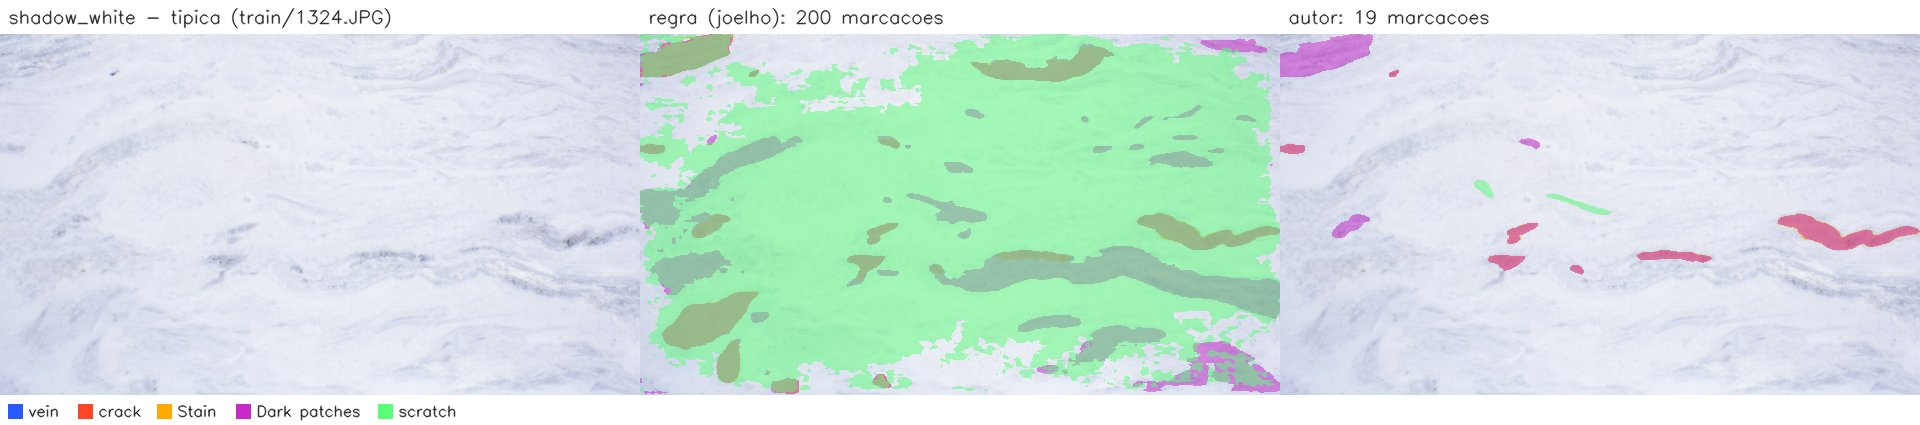
\includegraphics[width=\textwidth]{exemplo_shadow_white_tipica.jpg}

  \vspace{0.4cm}
  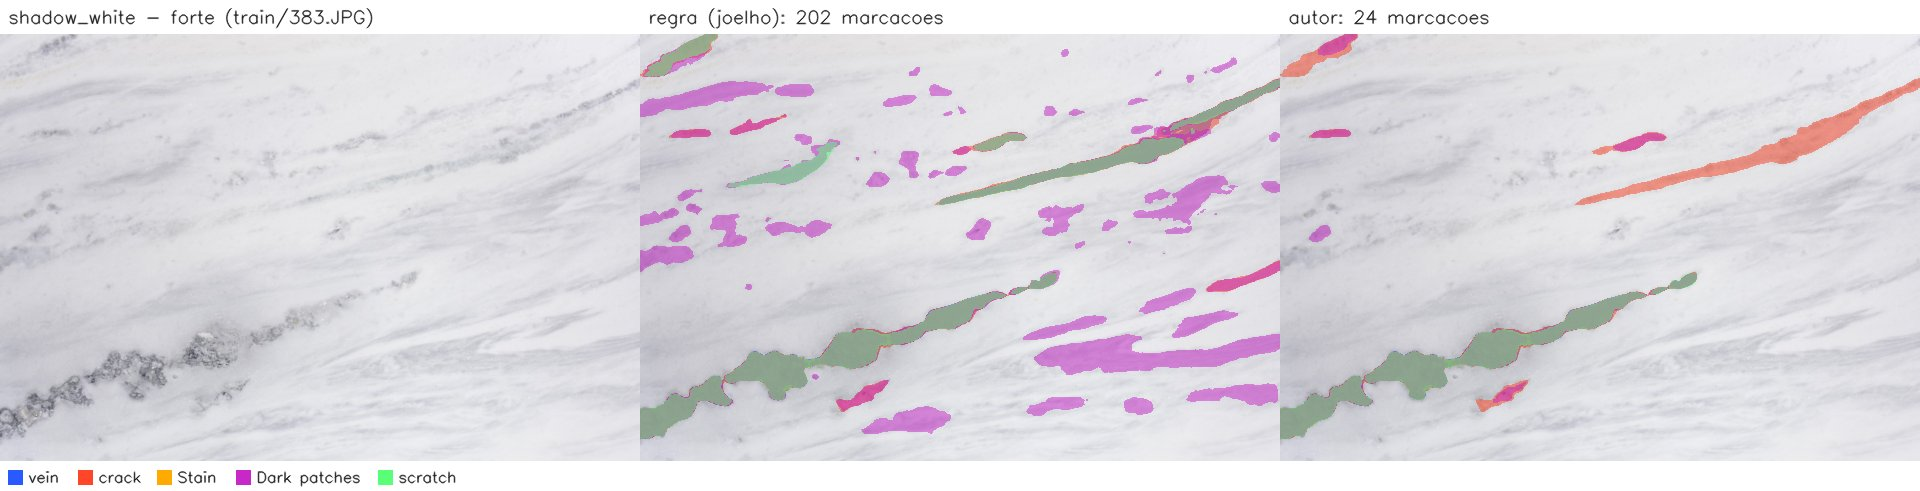
\includegraphics[width=\textwidth]{exemplo_shadow_white_forte.jpg}
  \legend{elaborado pelo autor, sobre imagens de \citeonline{dataset_araujo2023}}
\end{figure}

\begin{figure}[htbp]
  \caption{Regra e autor na \textit{siena\_white}: imagem típica (acima) e forte (abaixo).}
  \label{fig:ex_ap_siena_white}
  \centering
  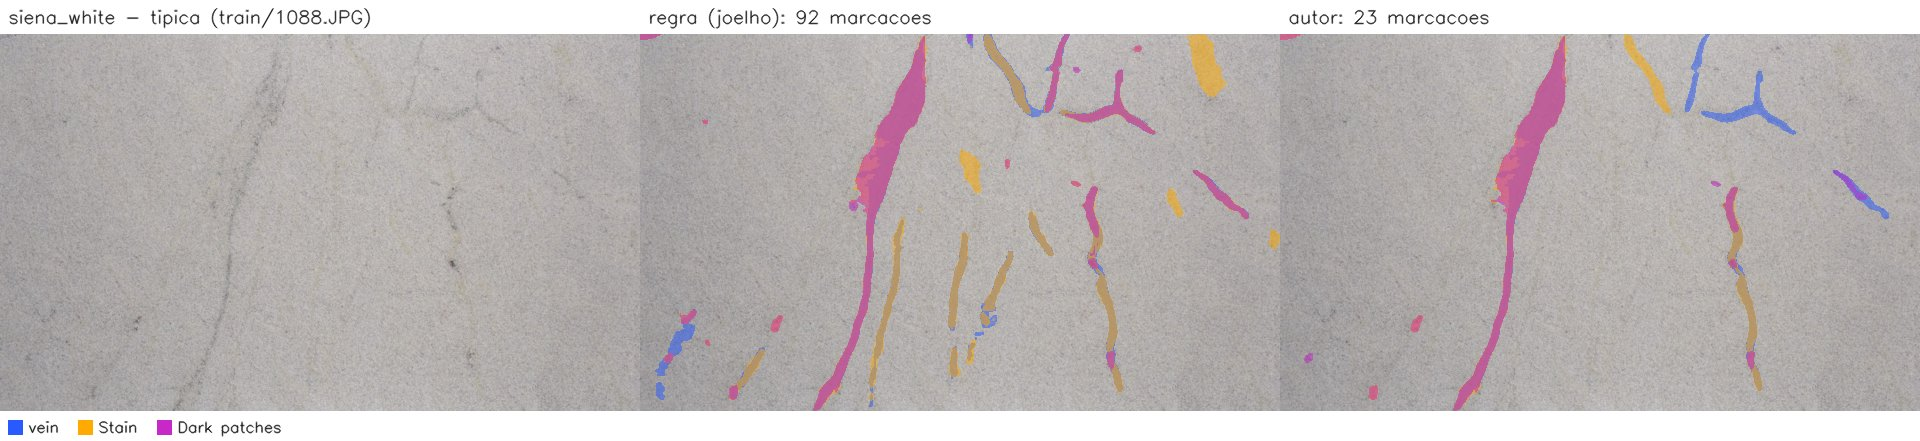
\includegraphics[width=\textwidth]{exemplo_siena_white_tipica.jpg}

  \vspace{0.4cm}
  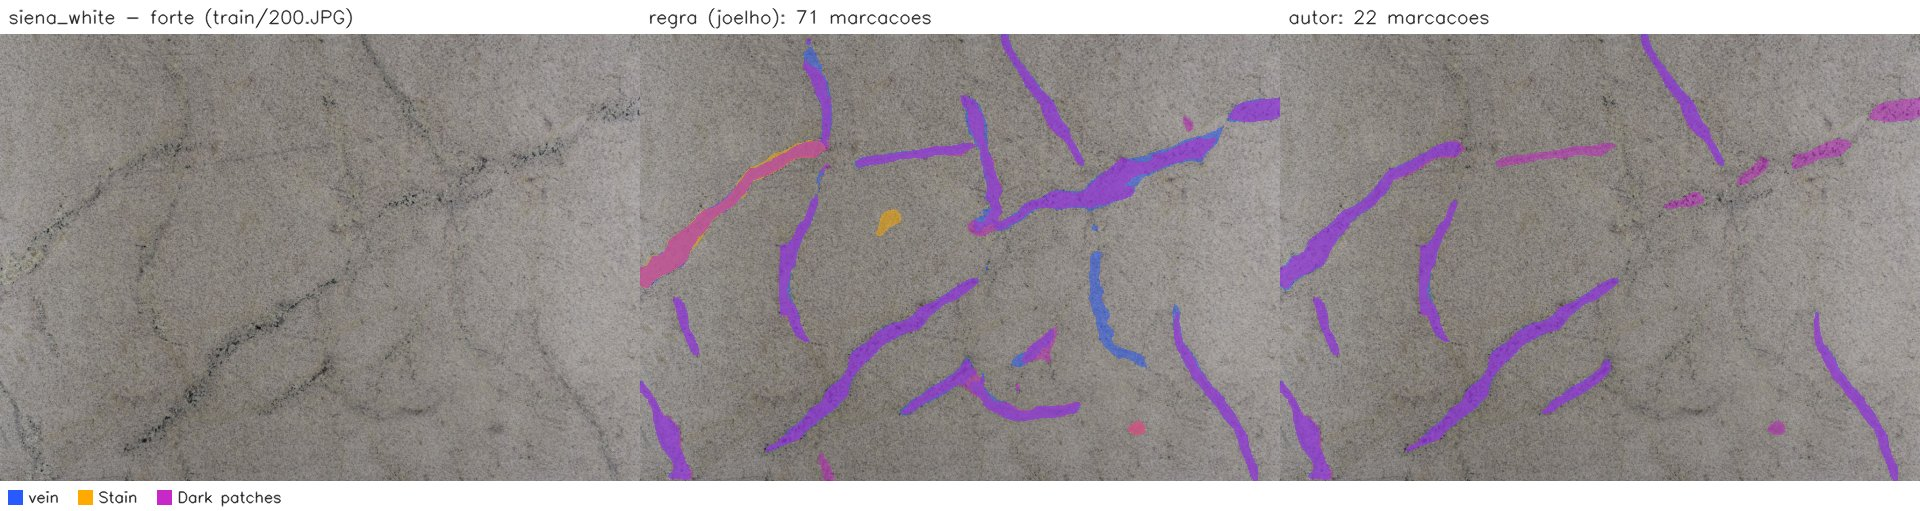
\includegraphics[width=\textwidth]{exemplo_siena_white_forte.jpg}
  \legend{elaborado pelo autor, sobre imagens de \citeonline{dataset_araujo2023}}
\end{figure}

\begin{figure}[htbp]
  \caption{Regra e autor na \textit{ubatuba\_green}: imagem típica (acima) e forte (abaixo).}
  \label{fig:ex_ap_ubatuba_green}
  \centering
  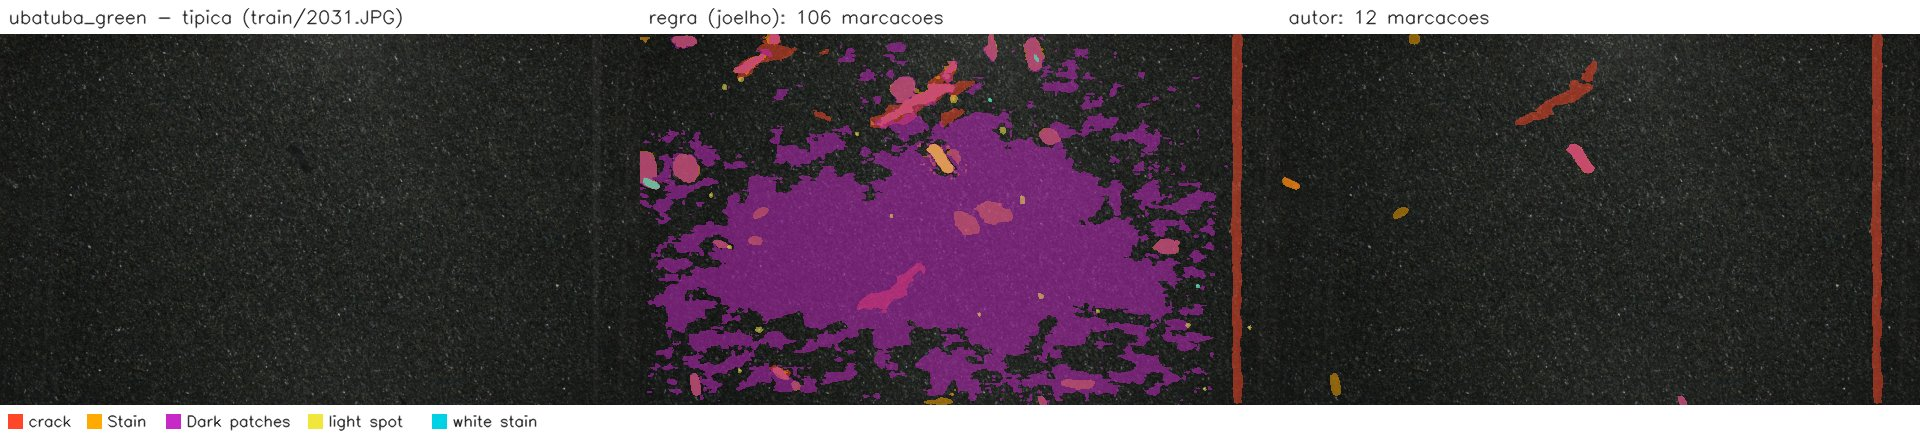
\includegraphics[width=\textwidth]{exemplo_ubatuba_green_tipica.jpg}

  \vspace{0.4cm}
  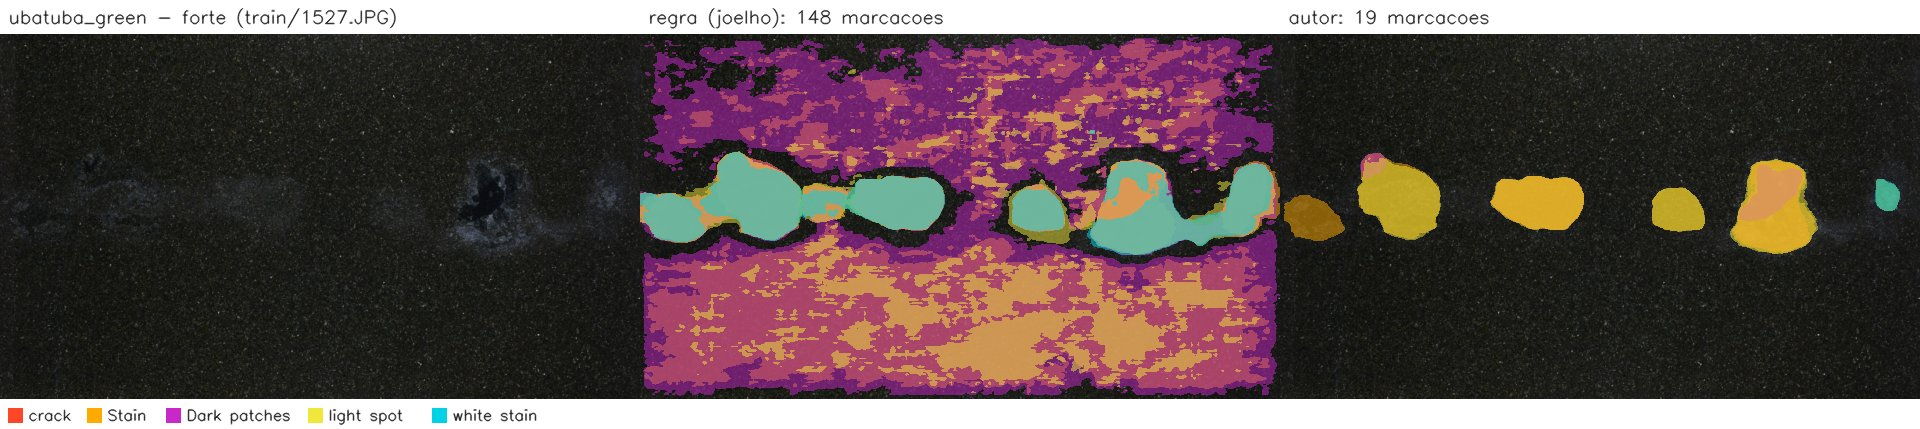
\includegraphics[width=\textwidth]{exemplo_ubatuba_green_forte.jpg}
  \legend{elaborado pelo autor, sobre imagens de \citeonline{dataset_araujo2023}}
\end{figure}

\begin{figure}[htbp]
  \caption{Regra e autor na \textit{white\_mirage}$^{\dagger}$: imagem típica (acima) e forte (abaixo).}
  \label{fig:ex_ap_white_mirage}
  \centering
  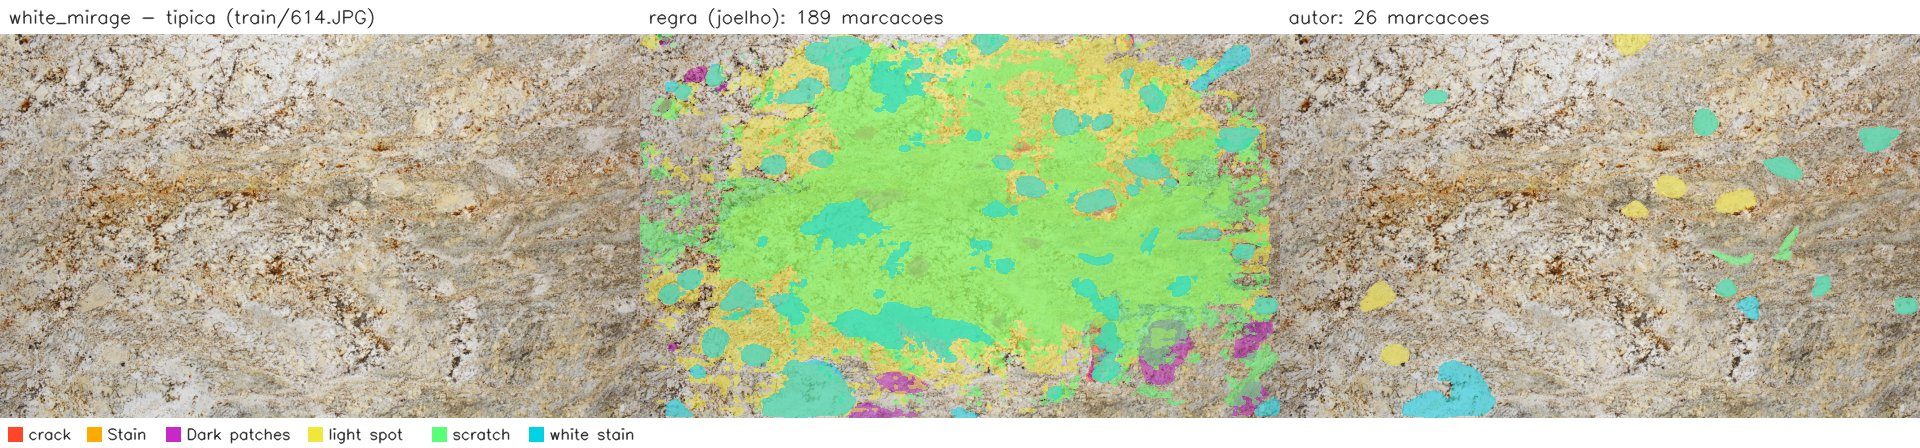
\includegraphics[width=\textwidth]{exemplo_white_mirage_tipica.jpg}

  \vspace{0.4cm}
  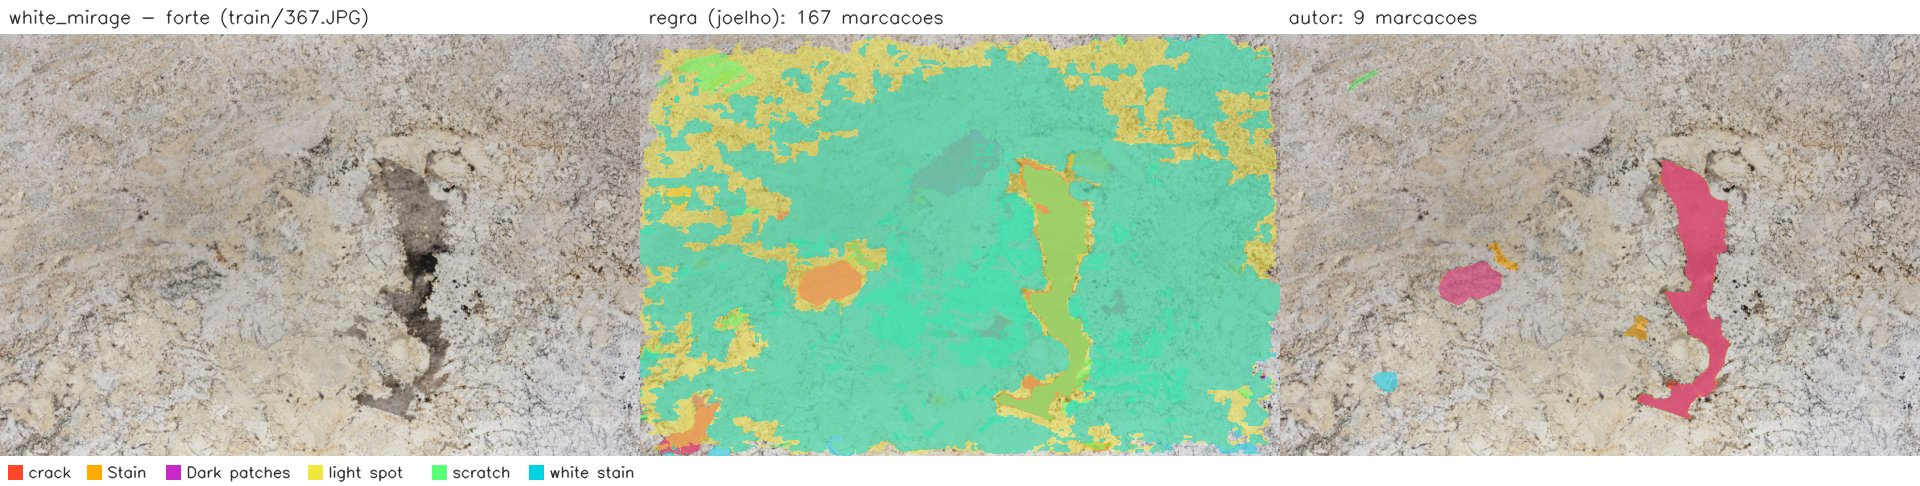
\includegraphics[width=\textwidth]{exemplo_white_mirage_forte.jpg}
  \legend{elaborado pelo autor, sobre imagens de \citeonline{dataset_araujo2023}}
\end{figure}

\begin{figure}[htbp]
  \caption{Regra e autor na \textit{white\_olympus}: imagem típica (acima) e forte (abaixo).}
  \label{fig:ex_ap_white_olympus}
  \centering
  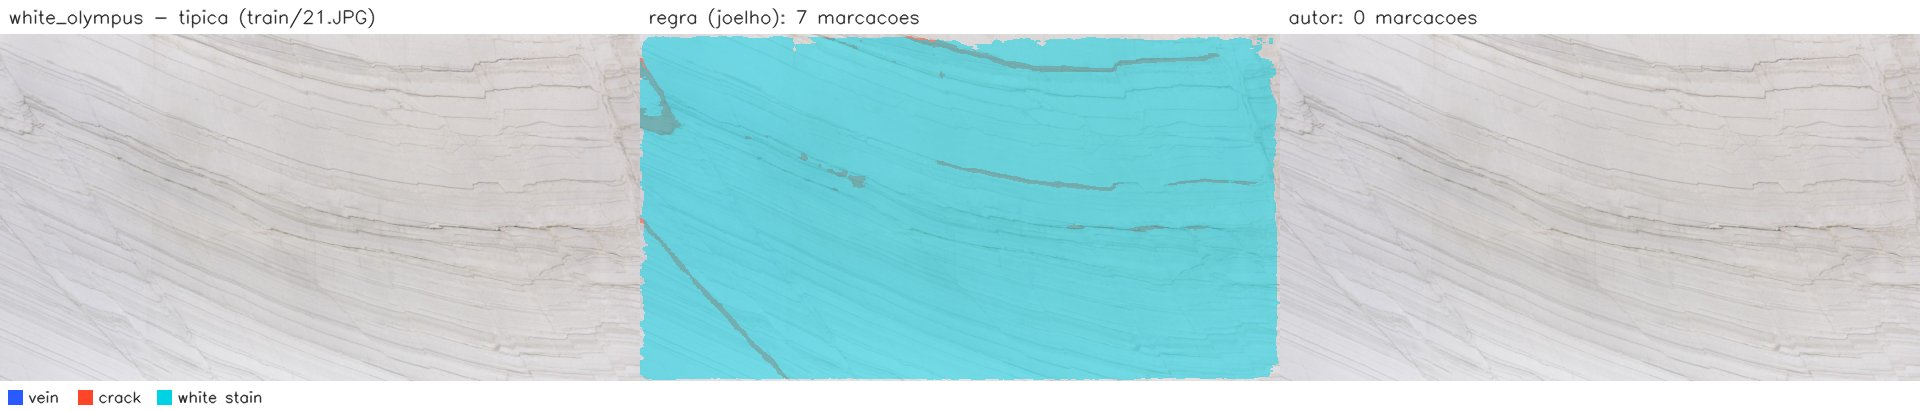
\includegraphics[width=\textwidth]{exemplo_white_olympus_tipica.jpg}

  \vspace{0.4cm}
  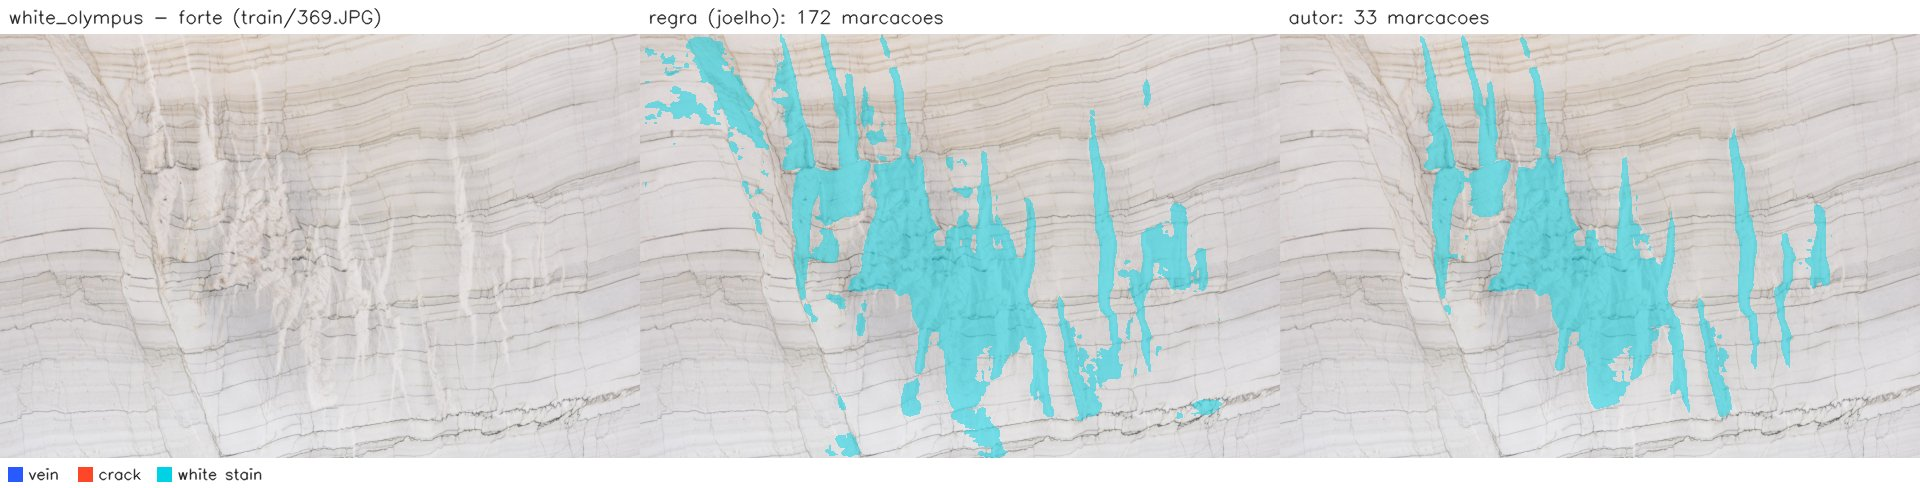
\includegraphics[width=\textwidth]{exemplo_white_olympus_forte.jpg}
  \legend{elaborado pelo autor, sobre imagens de \citeonline{dataset_araujo2023}}
\end{figure}
